\documentclass[a4paper]{exam}

\usepackage{amsmath,amssymb, amsthm}
\usepackage{geometry}
\usepackage{graphicx}
\usepackage{hyperref}
\usepackage{xcolor}
\usepackage{wasysym}

\usepackage{xcolor}
\usepackage{wasysym}


\usepackage{tikz}
\usepackage{tikz-qtree}

\usetikzlibrary{automata, positioning, arrows}
\tikzset{
  ->,  % makes the edges directed
  >=stealth, % makes the arrow heads bold
  node distance=2cm, % specifies the minimum distance between two nodes. 
  every state/.style={thick, fill=gray!10}, % sets the properties for each ’state’ node
  initial text=$ $, % sets the text that appears on the start arrow 
}
% Header and footer.
\pagestyle{headandfoot}
\runningheadrule
\runningfootrule
\runningheader{CS 212}{HW 02: Pumping Lemma, Context Free Languages}{Fall 2026}
\runningfooter{}{Page \thepage\ of \numpages}{}
\firstpageheader{}{}{}


\newcommand{\shuffle}{\textsc{shuffle}} % Use \shuffle typeset this operator.

\newtheorem{definition}{Definition}
\newtheorem{theorem}{Theorem}

\title{Homework 02: Pumping Lemma, Context Free Languages}
\author{CS 212 Nature of Computation\\Habib University\\
Muhammad Hamza Bin Tariq - mb09640\\% Please enter your name and ID here
Hassan Akhter - ha10609 % Please enter your name and ID here
}
\date{Fall 2026}

\boxedpoints


\printanswers % Uncomment this line

\begin{document}
\maketitle


\begin{questions}

	\question[10]
	\begin{definition}[Shuffle Operator]
		Let $L \subseteq \{0,1\}^*$ be a some language. The operator $\shuffle$ is defined as, $\shuffle(L) = \{w\in \{0,1\}^*\mid \exists x \in L \;s.t. \; w \text{ is obtained by shuffling the characters of } x\}$. More formally, $\shuffle(L) = \{w = w_1w_2\dots w_n\in \{0,1\}^*\mid \exists x = x_1x_2 \dots x_n \in L, \;s.t.\; \forall w_i !\exists x_j : w_i = x_j\}$.
	\end{definition}

	In HW1 we saw that if $L$ is a regular then $\shuffle(L)$ isn't necessarily regular. For this we showed that $\shuffle((01)^+)$ is not regular. But for regular $L$ is $\shuffle(L)$ always context free?

	Prove or disprove the following claim: $\shuffle((01)^+)$ is context free.

	\begin{solution}
		% Enter your solution here.
		The language $(01)^+$ is the language in which there is at least one $01$, or more in the fashion $010101$. Basically a language with an equal number of 0's and 1's in an alternating fashion.\\
		The $\shuffle()$ operator simply rearranges them in an arbitrary order, but the number of 1's and 0's stay the same.\\
		Lets say that we can construct a CFG $M(V,\Sigma, R, S)$ for the language $\shuffle((01)^+)$, such that:
		\begin{itemize}
			\item $V = \{S,A\}$
			\item $\Sigma = \{0,1\}$
			\item $R:$
			      \begin{itemize}
				      \item $S \rightarrow 1A0A \mid 0A1A$
				      \item $A \rightarrow 1A0A \mid 0A1A \mid \epsilon$
			      \end{itemize}
		\end{itemize}
		This ensures that it'll only accept strings with the same number of 0's and 1's in any order, the empty string is rejected, so there must be at least one 1 and one 0.\\
		Since a CFG can be formed for the $\shuffle((01)^+)$, therefore the language is context free.
	\end{solution}




	\question Your friend Abbas is in a Tom and Jerry-esque situation with a rat. Where he tries to catch the rat and the rat keeps outsmarting him. To taunt Abbas, every time the rat runs out to steal some cheese it yells out its catchphrase which is of form ``\emph{RRRRRAAAAATTTT}'' given by the RegEx $R^+A^+T^+$. Now Abbas, in a very Wile e Coyote-like fashion makes a contraption to catch the rat. The contraption has a DFA that recognizes the rat's catch phrase in order to detect the rat running around. The rat being much smarter than Abbas decides to modify its catchphrase slightly such that such that it's catchphrase is no longer regular, so its not detected by Abbas's machine. The new catch phrase is defined as $R^iA^jT^k$ where $i,j,k \in \mathbb{Z}^+$ and $i \neq 1$ or $j = k$.
	\begin{parts}
		\part[10] The rat graduated Habib University in 2021 with a CS degree, back in those days Nature of Computation was not a mandatory course. Due to this the rat doesn't know the pumping lemma.
		Without using pumping lemma show that the following language $L_R$ is not regular:
		$L_R = \{R^iA^jT^k|\; i,j,k \in \mathbb{Z}^+ \text{ and } i \neq 1 \text{ or } j = k\}$.
		\begin{solution}
			% Enter solution here
			Regular languages are closed under intersection. Consider the language:

			$$L = RA^+T^+$$
		\end{solution}

		\part[10] Abbas however has taken the Nature of Computation course, he knows that the set of context free languages is a superset of regular languages. He conjectures that the new language the rat is using to taunt him might be context free and he may be able to make \href{https://en.wikipedia.org/wiki/Pushdown_automaton}{a different model of computation} for it. Prove or disprove the claim that the language,
		$L_R = \{R^iA^jT^k|\; i,j,k \in \mathbb{Z}^+ \text{ and } i \neq 1 \text{ or } j = k\}$, is context-free.
		\begin{solution}
			% Enter solution here
			We can prove that the claim is true by making a PDA for the language $L_R$\\
			Let $L_1$ be a language such that $L_1 = \{R^iA^jT^k\mid i,j,k \in \mathbb{Z}^{+} \text{ and } i\neq 1\}$\\
			And let $L_2$ be a language such that $L_2 = \{R^iA^jT^k\mid i,j,k \in \mathbb{Z}^{+} \text{ and } j = k\}$\\
			$L_R$ is the union of the two languages $L_1$ and $L_2$\\
			$L_R = L_1 \cup L_2$\\
			The PDA of $L_1$ can be constructed, and is shown below:\\
			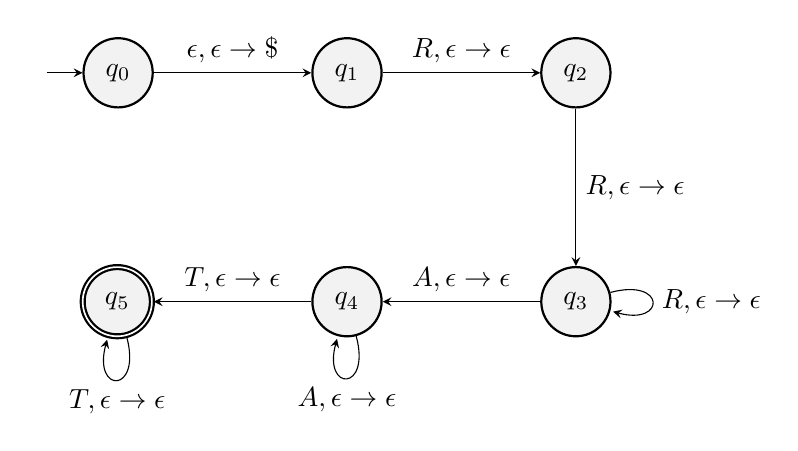
\begin{tikzpicture}
				% Row 1 (Left to Right)
				\node[state, initial] (q0) {$q_0$};
				\node[state, right=2cm of q0] (q1) {$q_1$};
				\node[state, right=2cm of q1] (q2) {$q_2$};

				% Row 2 (Right to Left, directly below Row 1)
				\node[state, below=2cm of q2] (q3) {$q_3$};
				\node[state, left=2cm of q3] (q4) {$q_4$};
				\node[state, accepting, left=2cm of q4] (q5) {$q_5$};

				\path
				(q0) edge node[above] {$\epsilon, \epsilon \to \$$} (q1)
				(q1) edge node[above] {$R, \epsilon \to \epsilon$} (q2)
				(q2) edge node[right] {$R, \epsilon \to \epsilon$} (q3)
				(q3) edge[loop right] node {$R, \epsilon \to \epsilon$} (q3)
				edge node[above] {$A, \epsilon \to \epsilon$} (q4)
				(q4) edge[loop below] node {$A, \epsilon \to \epsilon$} (q4)
				edge node[above] {$T, \epsilon \to \epsilon$} (q5)
				(q5) edge[loop below] node {$T, \epsilon \to \epsilon$} (q5);
			\end{tikzpicture}\\

			And the PDA of $L_2$ can also be constructed as shown below:\\
			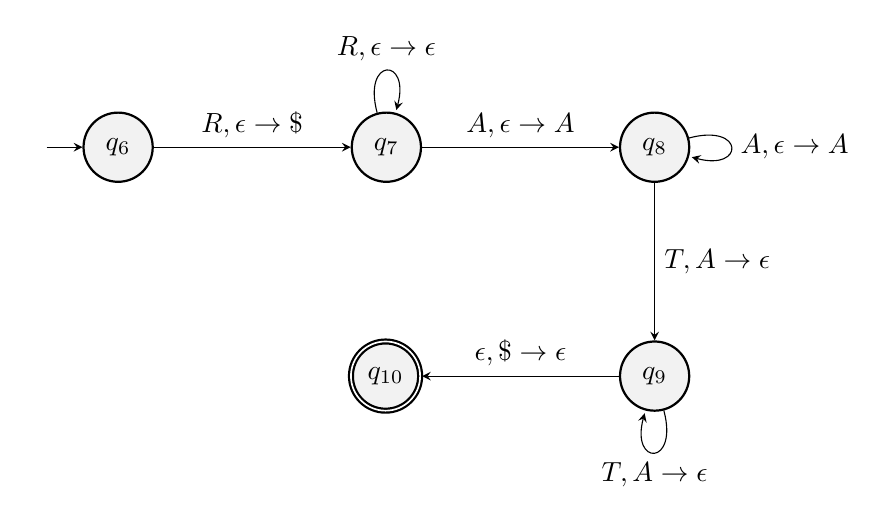
\begin{tikzpicture}
				% Row 1 (Left to Right)
				\node[state, initial] (q6) {$q_6$};
				\node[state, right=2.5cm of q6] (q7) {$q_7$};
				\node[state, right=2.5cm of q7] (q8) {$q_8$};

				% Row 2 (Right to Left, directly below Row 1)
				\node[state, below=2cm of q8] (q9) {$q_9$};
				\node[state, accepting, left=2.5cm of q9] (q10) {$q_{10}$};

				\path
				(q6) edge node[above] {$R, \epsilon \to \$$} (q7)
				(q7) edge[loop above] node {$R, \epsilon \to \epsilon$} (q7)
				edge node[above] {$A, \epsilon \to A$} (q8)
				(q8) edge[loop right] node {$A, \epsilon \to A$} (q8)
				edge node[right] {$T, A \to \epsilon$} (q9)
				(q9) edge[loop below] node {$T, A \to \epsilon$} (q9)
				edge node[above] {$\epsilon, \$ \to \epsilon$} (q10);
			\end{tikzpicture}\\\\
			Combining the two to form a union between $L_1 \text{ and } L_2$, we get the PDA of $L_R$ which is shown below.\\
			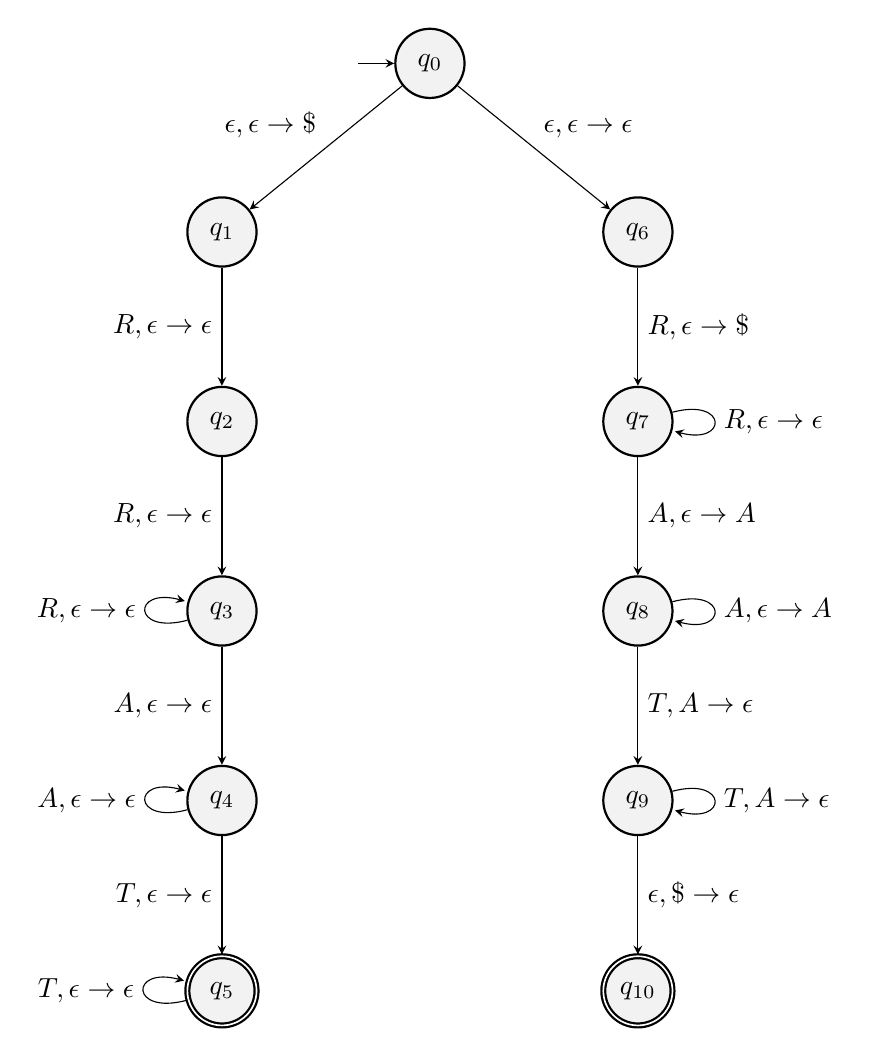
\begin{tikzpicture}
				% Start state at the top center
				\node[state, initial] (q0) {$q_0$};

				% Branch 1 (L1) - Flows vertically down the left side
				\node[state, below left=1.5cm and 2cm of q0] (q1) {$q_1$};
				\node[state, below=1.5cm of q1] (q2) {$q_2$};
				\node[state, below=1.5cm of q2] (q3) {$q_3$};
				\node[state, below=1.5cm of q3] (q4) {$q_4$};
				\node[state, accepting, below=1.5cm of q4] (q5) {$q_5$};

				% Branch 2 (L2) - Flows vertically down the right side
				\node[state, below right=1.5cm and 2cm of q0] (q6) {$q_6$};
				\node[state, below=1.5cm of q6] (q7) {$q_7$};
				\node[state, below=1.5cm of q7] (q8) {$q_8$};
				\node[state, below=1.5cm of q8] (q9) {$q_9$};
				\node[state, accepting, below=1.5cm of q9] (q10) {$q_{10}$};

				% Transitions
				\path
				% Branching from start
				(q0) edge node[above left] {$\epsilon, \epsilon \to \$$} (q1)
				edge node[above right] {$\epsilon, \epsilon \to \epsilon$} (q6)

				% L1 Transitions (Left Side)
				(q1) edge node[left] {$R, \epsilon \to \epsilon$} (q2)
				(q2) edge node[left] {$R, \epsilon \to \epsilon$} (q3)
				(q3) edge[loop left] node {$R, \epsilon \to \epsilon$} (q3)
				edge node[left] {$A, \epsilon \to \epsilon$} (q4)
				(q4) edge[loop left] node {$A, \epsilon \to \epsilon$} (q4)
				edge node[left] {$T, \epsilon \to \epsilon$} (q5)
				(q5) edge[loop left] node {$T, \epsilon \to \epsilon$} (q5)

				% L2 Transitions (Right Side)
				(q6) edge node[right] {$R, \epsilon \to \$$} (q7)
				(q7) edge[loop right] node {$R, \epsilon \to \epsilon$} (q7)
				edge node[right] {$A, \epsilon \to A$} (q8)
				(q8) edge[loop right] node {$A, \epsilon \to A$} (q8)
				edge node[right] {$T, A \to \epsilon$} (q9)
				(q9) edge[loop right] node {$T, A \to \epsilon$} (q9)
				edge node[right] {$\epsilon, \$ \to \epsilon$} (q10);
			\end{tikzpicture}\\
			Since we can construct a PDA for the language $L_R$, this proves that the language is indeed context free
		\end{solution}

	\end{parts}



	\question[10] Your friend Khubaib and Munawwar wish to evade taxes. Khubaib and Munawwar have decided to come up with a secret language to have all their embezzlement related correspondence in.
	As the tax auditor, uses a DFA to check for any suspicious activities, the language Khubaib and Munawwar come up with should not be regular.
	You were able to help them by giving them a language that you believe is not regular. You define the language as follows: $L_{\text{tax evasion}} = \{ w \in \{1, \smiley \}^* \mid w = w_1\smiley w_2\smiley \dots \smiley w_k \text{ for } k \geq 0, \text{ each } w_i \in 1^*, \text{ and } w_i \neq w_j \text{ for } i \neq j \}$. Prove or disprove that $L_{\text{tax evasion}}$ is not regular.

	% Use \smiley to write smile face emoji
	\begin{solution}

		Suppose that the language $L_{\text{tax evasion}}$ = $L_R$ is regular.

		Then by the pumping lemma, there exists a pumping length $p$ s.t.\ any string $w \in L_R$ with $|w| \geq p$ can be split into $xyz$ s.t.:
		\begin{itemize}
			\item[] $|xy| \leq p$
			\item[] $|y| > 0$
			\item[] $xy^iz \in L_R \quad \forall i \geq 0$
		\end{itemize}

		Consider the string $w = 1^p \smiley 1^{p + p!}$. $w_1 = 1^p$ and $w_2 = 1^{p + p!}$. Since $p \neq p + p!$, we have $w_1 \neq w_2$, so $w \in L_R$ and $|w| = 2p + p! + 1 \geq p$.

		Since $|xy| \leq p$ and $|y| > 0$, both $x$ and $y$ lie entirely within the first block $1^p$. Thus, $1^p = 1^{(p-m)} + 1^m$ where $y= 1^m$ and $1 \leq m \leq p$.

		Now pumping $y$ to $i$ we get $1^p = 1^{(p-m)} + 1^{(mi)}$. Factoring, $1^{(p+(i-1)m)} \smiley 1^{(p+p!)}$

		Consider that $i = 1 + \frac{p!}{m}$. This will be an integer because $m$ is a factor in $p!$ s.t $1 <= m <= p$, $\frac{p!}{m} = 1*2*...*(m-1)*m*(m+1)*...p / m$ divides cleanly.

		Therefore if we pump y to this integer, the resulting string is $1^{(p + (1 + \frac{p!}{m} - 1)m)} \smiley 1^{(p + p!)} = 1^{(p + p!)} \smiley 1^{(p + p!)}$.

		In this new pumped string, ($w_1 = w_2 = 1^{p + p!}$), which violates $w_i \neq w_j$ for $i \neq j$.

		Therefore, $xy^iz \notin L_R$, and we can conclude that the language $L_R$ is not regular as proven by contradicting the Pumping lemma.
	\end{solution}


\end{questions}

\end{document}

%%% Local Variables:
%%% mode: latex
%%% TeX-master: t
%%% End:


